\section{NS}%
\label{sec:ns}

\begin{frame}
	\frametitle{Graphs are everywhere!}
	
	\begin{center}
		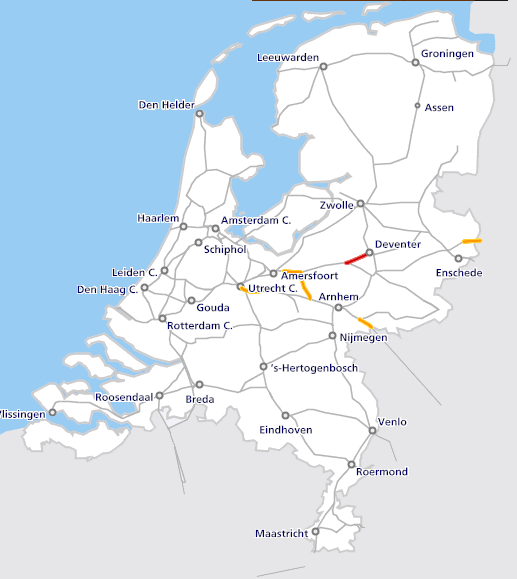
\includegraphics[width=0.35\textwidth]{figures/ns.png}\\
		\hspace*{15pt}\hbox{\scriptsize Screenshot by: \thinspace{\itshape Stefan Hugtenburg}}\\
		\hspace*{15pt}\hbox{\scriptsize Taken from: \url{https://ns.nl}}
	\end{center}
\end{frame}

\begin{frame}
	\frametitle{Rail networks}
	
	\begin{overlayarea}{\textwidth}{\textheight}
			\begin{problemblock}{Questions to ask}
				The NS maintains a large network of railroads in the Netherlands. There are many questions related to this:
				\begin{itemize}
					\item \alert<5>{What cities can you reach by train?}
						\pause
					\item \alert<6>{What is the quickest way to get from A to B?}
						\pause
					\item \alert<7>{What is the best way to connect new stations to the network?}
						\pause
					\item \alert<8>{How can we quickly tour the entire country?}
				\end{itemize}
			\end{problemblock}
			\only<5>{
			\begin{answerblock}{Traversals}
				This we can figure out by traversing the graph, which we will do today.
			\end{answerblock}
		}
		\only<6>{
			\begin{answerblock}{Shortest path algorithms}
				This we can figure out by using a shortest path algorithm (next Monday).
			\end{answerblock}
		}
		\only<7>{
			\begin{answerblock}{Shortest path algorithms}
				This we can figure out by using a Minimum Spanning Tree (next Tuesday).
			\end{answerblock}
		}
		\only<8>{
			\begin{alertblock}{TSP}
				This we cannot figure out! It's called the Travelling Salesman Problem (Monday two weeks from now)
			\end{alertblock}
		}
	\end{overlayarea}
\end{frame}

